\chapter{Calibration to the SPX surface}
\label{cap:calibrazione}

This chapter fits two models to the SPX implied-volatility surface (snapshot of 6 November 2026, 22:13): a single
Heston parameter set for the whole surface and one SABR per expiry. Before the real data, we check on synthetic data,
with tolerances fixed in advance, that the procedure recovers known parameters. At the end we check that the surface
contains no static arbitrage. Code: \code{src/qpricer/calibration.py}; numbers: \code{scripts/run\_calibration.py} and
\code{scripts/phase5\_gates.py}.

\section{What calibrating means}
Calibrating means choosing the parameters $p$ so that the model reproduces the market as closely as possible. It is a
\textbf{nonlinear least-squares} problem:
\begin{equation}\label{eq:cal-ls}
\hat p=\arg\min_p\ \tfrac12\sum_{i=1}^n r_i(p)^2 ,
\end{equation}
where $r_i$ is the weighted \emph{residual} of quote $i$ and $\tfrac12\sum_ir_i^2$ is the \emph{cost}. Three
questions organize the chapter: \emph{what} is compared and with what weight; \emph{how} the model is computed inside
the optimizer without numerical error disturbing the search; \emph{how far} the result can be trusted.

\section{The targets}
\subsection{Bid, ask and mid volatilities}
We start from the OTM surface of Chapter~\ref{cap:dati}: 7625 quotes on 39 expiries, from $T=0.019$ to $T=1.61$
years. The discount factors of the short expiries have already been replaced with a rate curve and the forwards
re-estimated (Section~\ref{sec:breve-termine}).

For each quote $i$ the bid, ask and mid are inverted with Black, and the \textbf{half-spread in volatility}
$h_i=\tfrac12(\sigma^a_i-\sigma^b_i)$ is defined. For an OTM option the intrinsic value is zero, so the bid volatility
exists as soon as the bid is positive.

Notation:
\[
k=\ln(K/F),\qquad s=\sigma\sqrt T,\qquad d_1=-\frac ks+\frac s2,\qquad d_2=d_1-s .
\]
The model prices are \emph{normalized} ($F=\DF=1$, strike $e^k$): Heston and SABR with $\beta=1$ depend only on
$K/F$. The normalized vega is $\vega=\varphi(d_1)\sqrt T$.

\subsection{Delta band and thinning}
A quote enters if the mid volatility exists, if the mid is worth at least 0.50 (10 minimum SPX ticks) and if
$|d_1(\sigma^m_i)|\le z_5=\Phi^{-1}(0.95)=1.6449$, that is, between the 5-delta put and call. Beyond 5$\Delta$ the
options are worth a few ticks, the spread is a large fraction of the price and the volatility is almost undetermined.

Then we \textbf{thin}: 25 targets equally spaced in $d_1$ between $-z_5$ and $z_5$ are fixed, for each one the
not-yet-used quote with the closest $d_1$ is taken, and the put and the call closest to $k=0$ are always added. Each
expiry thus has 25--27 quotes.

\begin{perche}[title={Why thin, and why 25}]
\begin{itemize}
\item A smile within the band has about 4--5 ``shape numbers'' (level, slope, curvature, wing slopes): 25 points give
at least 5 per number.
\item Adjacent strikes 5 points apart differ by $\Delta k\approx7\times10^{-4}\ll s$: they are quoted by the same
market maker and their errors are not independent. They add weight, not information. Targets 0.14 apart in $d_1$ make
the independent-errors assumption on which the error bars rest more credible.
\item Without thinning, the weeklies (hundreds of strikes) would dominate the sum \eqref{eq:cal-ls}.
\end{itemize}
\end{perche}

\subsection{The Heston window}
Heston is calibrated only on the 21 expiries with $T\ge0.1$; the 18 shortest are left \textbf{out of sample}. The
reason, derived in Section~\ref{sec:cal-skew}, is that Heston has a single time scale, $1/\kappa$, and cannot
reproduce both the skew of the weeklies and that of the long expiries. We fit the expiries that matter for the
autocallable (0.1--1.6 years) and \emph{measure} the error on the others. SABR is calibrated on all expiries, one at a
time.

\begin{progetto}[title={In the qpricer project: the targets}]
7625 OTM quotes $\to$ 5806 in the band $\to$ 1029 after thinning $\to$ 565 Heston residuals on the 21 expiries with
$T\ge0.1$, plus 464 out-of-sample quotes. Functions \code{in\_band} and \code{thin}.
\end{progetto}

\section{The objective function}
\subsection{Volatility residuals}
The Heston residual is
\begin{equation}\label{eq:cal-res}
r_i(p)=w_i\big[\sigma^H_i(p)-\sigma^m_i\big],\qquad w_i=\frac{1}{\max(h_i,\,h_{\min})},\qquad h_{\min}=0.001 ,
\end{equation}
with $\sigma^H_i$ the implied volatility of the Heston price. With this weight $|r_i|\le1$ means that the model is
\emph{inside} the bid/ask. The \textbf{floor} $h_{\min}$ (0.1 vol points) prevents the very tight quotes from
dominating: it is active on 60.9\% of the thinned quotes (median half-spread 0.078 vol points).

\subsection{Equivalence with vega-weighted prices}
\noindent\textbf{Step 1.} With $\Delta=\sigma^H-\sigma^m$, expand the normalized Black price in $\sigma$:
\[
v(\sigma^H)-v(\sigma^m)=\vega^m\Delta+\tfrac12\,\partial_\sigma\vega^m\,\Delta^2+O(\Delta^3).
\]
\noindent\textbf{Step 2.} Differentiating $\vega=\varphi(d_1)\sqrt T$ gives $\partial_\sigma\vega/\vega=d_1d_2/\sigma$,
with $d_1d_2=k^2/s^2-s^2/4$.

\noindent\textbf{Step 3.} Dividing by $\vega^m$:
\begin{equation}\label{eq:cal-prezzo-vol}
\frac{v^H-v^m}{\vega^m}=\Delta\Big[1+\frac{d_1d_2}{2\sigma^m}\,\Delta\Big]+O(\Delta^3).
\end{equation}
\noindent\textbf{Step 4.} At first order the price residual divided by vega \emph{is} the volatility residual:
minimizing $\sum w_i^2\Delta_i^2$ is equivalent to weighting the price errors by $w_i^2/(\vega^m_i)^2$. The Jacobians
also coincide at first order, so near the optimum the minimum and the standard errors are the same. At the edge of
the band, with $\sigma=0.2$ and $\Delta=0.3$ vol points, the correction is about 2\% (estimate).

\begin{perche}[title={Why volatilities, then}]
Far from the optimum $\Delta$ is not small: in the wings $d_1d_2$ is large and the price is convex and steep in
$\sigma$, so the price residuals blow up and dominate the first iterations. Volatility residuals stay bounded, and the
quantity to report at the end is precisely a volatility error.
\end{perche}

\subsection{The fallback}
With extreme trial parameters the Heston price may not be invertible (too small, or set to zero because the strike
falls outside the COS interval). A \code{NaN} would stop the optimizer. On those quotes the first-order equivalent
residual is used instead:
\begin{equation}\label{eq:cal-ripiego}
r_i=w_i\,\frac{v^H_i-v^m_i}{\vega^m_i},\qquad \vega^m_i\ \text{computed at } \sigma^m_i .
\end{equation}
The market vega always exists. Fallbacks are counted; at the optimum there are none.

\begin{progetto}
\code{heston\_residuals} forms \eqref{eq:cal-ripiego} and replaces it with \eqref{eq:cal-res} where the inversion
succeeds; with \code{kind="price"} it returns price residuals only. Started from the same points, this second objective
function ends up within 0.83 standard errors of the optimum on the real data (0.48 on the synthetic data S1): the
numerical confirmation of \eqref{eq:cal-prezzo-vol}.
\end{progetto}

\section{COS inside an optimizer}
\subsection{\texorpdfstring{Why freeze $(N,L)$}{Why freeze (N,L)}}
The self-checking COS of Chapter~\ref{cap:heston} chooses $(N,L)$ by itself, and the choice depends on $p$: the price
is a \emph{piecewise} function of the parameters, with jumps of the order of $10^{-9}F$. The optimizer estimates the
Jacobian with finite differences of relative step $10^{-6}$. If the step crosses a level change, it measures the jump
and not the slope: an error of about $10^{-9}/10^{-6}=10^{-3}$ on the derivative (estimate), erratic steps, premature
stops.

So $(N,L)$ is frozen for the whole fit, and $r(p)$ becomes smooth. But the fixed value must be accurate
\emph{wherever} the optimizer may go, that is, over the whole constraint box.

\subsection{The a-priori budget}
Before the fit a criterion is fixed: a \textbf{price error in units of market vega},
\begin{equation}\label{eq:cal-budget}
e_{\vega}=\max_i\frac{\big|v^{\mathrm{COS}}_i-v^{\mathrm{Lewis}}_i\big|}{\vega^m_i}\le10^{-5},
\end{equation}
with Lewis as the independent reference. By \eqref{eq:cal-prezzo-vol} it is the first-order volatility error
\emph{where the model is close to the market}, the only place where an error moves the optimum; it has the scale of
the fallback and is defined even where the model volatility does not exist. $10^{-5}$ is 0.001 vol points: 37 times
below the smallest half-spread, 100 times below $h_{\min}$. It is checked on the 565 Heston quotes at the 32 vertices
of the box and at 128 interior Sobol points.

Pairs tried: $(8192,48)$ gives $3.7\times10^{-5}$ and $(16384,80)$ gives $2.0\times10^{-5}$, both over budget;
$(16384,64)$ gives $9.21\times10^{-6}$ and is chosen. The worst vertex is
\[
(v_0,\kappa,\theta,\xi,\rho)=(0.01,\,0.5,\,0.01,\,3,\,-0.99).
\]
Freezing $(N,L)$ per expiry would save less than 10\%: it is the long expiries that need more terms.

\begin{attenzione}[title={The budget is not a volatility accuracy}]
At the worst vertex the direct error $|\sigma^{\mathrm{COS}}-\sigma^{\mathrm{Lewis}}|$ is $2.48\times10^{-3}$, and
over the whole box it reaches $6.41\times10^{-3}$: only at the vertices with $\xi=3$, $\rho=-0.99$ and on the OTM
calls. There the model volatility is 2--5\% against the market's 13--15\%, and the model vega is $10^{-4}$ to
$10^{-11}$ times the market one: a tiny price error becomes a large volatility error, on a residual that is worth
about 10 vol points anyway. The volatility accuracy that matters is the one at the optimum, checked after the fit.
\end{attenzione}

\subsection{Why the box was narrowed}
The initial design had $v_0,\theta\in[10^{-4},1]$, $\kappa\in[10^{-3},20]$, $\xi\in[0.01,5]$ and COS fixed at
$(1024,12)$. The check against Lewis refuted it.
\begin{itemize}
\item At a plausible point, $(0.03,2,0.04,1,-0.7)$, $L=12$ gives a volatility error of $9.9\times10^{-5}$ ($L=18$:
$9.8\times10^{-7}$).
\item On the original box no fixed pair up to $(4096,30)$ is accurate, and at 4 vertices ($v_0=\theta=10^{-4}$,
$\xi=5$) even the Lewis quadrature fails.
\item The difficult region has small $v_0,\theta$, small $\kappa$ and large $\xi$: $\ln(F_T/F)$ is extremely
leptokurtic, and COS ends up requiring $L\approx80$ with $N=16384$.
\end{itemize}
The production box is
\begin{equation}\label{eq:cal-box}
v_0,\theta\in[0.01,\,0.25],\quad \kappa\in[0.5,\,20],\quad \xi\in[0.01,\,3],\quad \rho\in[-0.99,\,0],
\end{equation}
that is, volatilities between 10\% and 50\%. $\kappa\ge0.5$ is also the edge of the identifiable region
($\kappa T_{\max}\approx0.8$), and with $\rho\le0$ the condition $\kappa-\rho\xi>0$ holds everywhere.

\begin{attenzione}[title={Isn't narrowing the constraints cheating? The check}]
The fit was repeated on the \emph{original} box, with the same pair $(16384,64)$, from 16 Sobol points and from 4
hostile starts (for example $v_0=\theta=10^{-3}$ with $\xi=4.5$, or $\kappa=0.01$). \textbf{20 starts out of 20} reach
the same $\hat p$ (cost equal to $4.7\times10^{-15}$ relative), and $\hat p$ lies \textbf{at least 38 standard errors
inside} the narrowed constraints. An independent check with its own pricer obtained the same. The narrowing does not
move the result; the check is re-run with \code{scripts/run\_calibration.py -{}-box note}.
\end{attenzione}

\begin{progetto}[title={In the qpricer project: frozen COS}]
After the fit COS and Lewis agree in volatility to $4.9\times10^{-13}$ on the 565 in-sample quotes and to
$7.0\times10^{-13}$ on the 464 out-of-sample ones. One residual evaluation costs 87\,ms; the fit with 16 starts takes
29.4\,s on 8 processes.
\end{progetto}

\section{The solver and the error bars}
\subsection{Trust region and multi-start}
We use \code{scipy.optimize.least\_squares} with the \textbf{TRF} method: at each step it linearizes
$r(p)\approx r+J\delta p$, minimizes the approximate cost within a ``trust region'' and enlarges or shrinks the region
according to the quality of the approximation; the box constraints are satisfied by construction. The finite-difference
step is $10^{-6}$ relative: the default one ($\approx1.5\times10^{-8}$) would run into the noise of the volatility
inversion ($\approx10^{-13}$), with relative errors on the derivative close to $10^{-4}$ (estimate).
\code{x\_scale='jac'} rescales parameters that differ by a factor of about 100.

We start from $16=2^4$ points of a \textbf{scrambled Sobol} sequence, with a fixed seed and independent of the data, in
the box
\[
\sqrt{v_0},\sqrt\theta\in[0.10,\,0.40],\quad \ln\kappa\in[\ln0.5,\,\ln8],\quad \ln\xi\in[\ln0.2,\,\ln3],\quad
\rho\in[-0.95,\,-0.2].
\]
$\hat p$ is the converged start with the lowest cost; the \textbf{basin} is the set of starts with cost within a
factor $1+10^{-4}$. A single start would not tell whether the minimum is unique.

\subsection{Standard errors from the Jacobian}
\noindent\textbf{Step 1.} Near the optimum $r(\hat p+\delta p)\approx r(\hat p)+J\delta p$.

\noindent\textbf{Step 2.} If the residuals are independent errors with a common variance, the latter is estimated from
the degrees of freedom:
\begin{equation}\label{eq:cal-s2}
s^2=\frac{2\,\text{cost}}{n-5}.
\end{equation}
\noindent\textbf{Step 3.} The normal equations give $\delta\hat p=-(J^\top J)^{-1}J^\top\varepsilon$, hence
\begin{equation}\label{eq:cal-cov}
C=s^2(J^\top J)^{-1},\qquad \SE_j=\sqrt{C_{jj}},\qquad R_{jk}=\frac{C_{jk}}{\SE_j\SE_k}.
\end{equation}
The inverse is computed with the SVD of $J$, discarding zero singular values. The SVD of $J\,\mathrm{diag}|\hat p|$
gives the relative condition number and the \emph{weakest direction}, the combination the data see worst.

\begin{attenzione}
These are \emph{curvature} standard errors: they hold if the model is right, the window is the chosen one and the
errors are independent. They say nothing about misspecification error.
\end{attenzione}

\subsection{Identifiability}
\label{sec:cal-ident}
\paragraph{\texorpdfstring{The $\kappa$--$\theta$ ridge.}{The kappa-theta ridge.}} The average ATM variance up to $T$
is
\begin{equation}\label{eq:cal-vbar}
\bar v(T)=\theta+(v_0-\theta)\frac{1-e^{-\kappa T}}{\kappa T}=v_0+\tfrac12\kappa(\theta-v_0)T-\tfrac16\kappa^2(\theta-v_0)T^2+\dots
\end{equation}
If all expiries have $\kappa T\ll1$, the data see only $v_0$ and the product $\kappa(\theta-v_0)$: the cost is almost
flat along a hyperbola, the \textbf{ridge}. If all have $\kappa T\gg1$, only $\theta$ and $(v_0-\theta)/\kappa$ are
seen. Separating $\kappa$ from $\theta$ requires expiries with $\kappa T\approx1$.

\paragraph{\texorpdfstring{$\rho$--$\xi$ and $\kappa$--$\xi$.}{rho-xi and kappa-xi.}} The skew is first order in
$\rho\xi$, the curvature second order in $\xi$: only the curvature separates $\rho$ from $\xi$. Moreover, for
$\kappa T\gg1$ the skew decays as $\rho\xi/(2\kappa\sqrt\theta\,T)$ (below): the long expiries see $\xi/\kappa$, and
a positive correlation between $\kappa$ and $\xi$ is expected.

\paragraph{Feller.} $\nu_F=2\kappa\theta/\xi^2$ is \emph{reported}, not imposed: it is not a box constraint, and
imposing it would ruin the skew. It does not matter for Fourier, it matters for Monte Carlo (Chapter~\ref{cap:mc}).

\subsection{The Heston ATM skew}
\label{sec:cal-skew}
From Chapter~\ref{cap:heston}, at first order in $\xi$: $V_H=V_B(\bar v)+\rho\xi J\,\partial_x\partial_\Sigma V_B$,
with $J$ from \eqref{eq:J} and $\Sigma=\bar vT$.

\noindent\textbf{Step 1.} Divide the price correction by the vega $\DF F\varphi(d_1)\sqrt T$:
\[
\partial_x\partial_\Sigma V_B=-\frac{\DF F\varphi(d_1)\,d_2}{2\Sigma}
\quad\Longrightarrow\quad
\delta\sigma=-\frac{\rho\xi J\,d_2}{2\Sigma\sqrt T}.
\]

\noindent\textbf{Step 2.} With $d_2=-k/\sqrt\Sigma-\sqrt\Sigma/2$ we have $\partial_kd_2=-1/\sqrt\Sigma$, hence
\begin{equation}\label{eq:cal-skew}
\psi_H(T):=\partial_k\sigma\big|_{k=0}=\frac{\rho\xi J(T)}{2\,\bar v^{3/2}T^2}.
\end{equation}
\noindent\textbf{Step 3.} For $v_0=\theta$, $J=\theta(T-\tau_\kappa)/\kappa$ with
$\tau_\kappa=(1-e^{-\kappa T})/\kappa$, and
\begin{equation}\label{eq:cal-g}
\frac{\psi_H(T)}{\psi_H(0)}=g(\kappa T),\qquad g(x)=\frac{2(x-1+e^{-x})}{x^2}=1-\frac x3+\frac{x^2}{12}-\dots
\end{equation}
For $T\to0$ the skew tends to the \emph{finite} value $\rho\xi/(4\sqrt{v_0})$; for $\kappa T\gg1$, $g\approx2/x$ and
$\psi_H\approx\rho\xi/(2\kappa\sqrt\theta\,T)$ decays as $1/T$.

\begin{idea}[title={Key idea: Heston has a single clock}]
The Heston skew is almost flat for $T\ll1/\kappa$ and decays as $1/T$ beyond: the only scale is $1/\kappa$. The SPX ATM
skew, according to the \emph{literature}, follows instead a power law of about $T^{-0.4}$ (Bayer--Friz--Gatheral
estimate the exponent 0.407 on a 2013 surface; it has not been measured on the project snapshot). If this held here,
from $T=0.019$ to $0.1$ the market skew would roughly double, while that of Heston with $\kappa=3$ would change by about
8\% (estimates). A $\kappa$ large enough to steepen the weeklies would flatten the long expiries.
\end{idea}
\eqref{eq:cal-skew} is first order in $\xi$, and the calibrated $\xi$ is large: it serves to understand the shape in
$T$, not to compute numbers.

\section{The synthetic test}
\subsection{Data and a-priori tolerances}
Data labelled \textbf{synthetic} are generated from true parameters $p^*$, on the actual Heston grid (565 quotes, with
their $k_i$, $T_j$, $w_i$), with noise $\sigma^{\mathrm{obs}}_i=\sigma^H_i(p^*)+\varepsilon_i$,
$\varepsilon_i\sim N(0,\sigma_\varepsilon^2)$, $\sigma_\varepsilon=0.003$. Two sets: \textbf{S1}, the GS set of
Chapter~\ref{cap:heston} ($v_0=\theta=0.0354$, $\kappa=1.3253$, $\xi=0.3877$, $\rho=-0.7165$; Feller violated,
$\nu_F=0.62$), and \textbf{S2} ($0.015,\,3,\,0.04,\,0.4,\,-0.7$; $\nu_F=1.5$). The seeds are fixed and never changed.

``Recovered'' must mean ``within the expected error'', and the expected error is computed at $p^*$, \emph{without} a
fit.

\noindent\textbf{Step 1.} The fit minimizes $\|W^{1/2}(\sigma(p)-\sigma^{\mathrm{obs}})\|^2$ with
$W=\mathrm{diag}(w_i^2)$. With $J_\sigma=\partial\sigma^H/\partial p$ at $p^*$, the linearized normal equations give
\[
\delta p=A^{-1}J_\sigma^\top W\varepsilon,\qquad A=J_\sigma^\top WJ_\sigma .
\]

\noindent\textbf{Step 2.} The noise has constant variance but the weights are not $1/\sigma_\varepsilon$, so the
\textbf{sandwich} form is needed:
\begin{equation}\label{eq:cal-sandwich}
\Sigma_p=\sigma_\varepsilon^2\,A^{-1}\big(J_\sigma^\top W^2J_\sigma\big)A^{-1},\qquad \SE_j=\sqrt{(\Sigma_p)_{jj}}.
\end{equation}
\noindent\textbf{Step 3.} At first order $\delta p$ is Gaussian: $D^2=\delta p^\top\Sigma_p^{-1}\delta p\sim\chi^2_5$.
The final residual is the noise projected out of a 5-dimensional space, so the RMSE is about
$\sigma_\varepsilon\sqrt{(n-5)/n}$ with standard deviation $\sigma_\varepsilon/\sqrt{2n}$, and the cost at $\hat p$
does not exceed the cost at $p^*$.

$\Sigma_p$ depends only on $p^*$, the grid, the weights and $\sigma_\varepsilon$: it is \emph{a priori}.

\subsection{The checks G1--G4}
Before any noisy fit, an \textbf{identifiability check}: $p^*_j\pm3\SE_j$ inside the constraints and
$3\SE_j\le0.5|p^*_j|$. Then:
\begin{itemize}
\item \textbf{G1}, without noise: every parameter recovered to $10^{-6}$ relative;
\item \textbf{G2}, with noise: $|\hat p_j-p^*_j|\le3\SE_j$ for every $j$ \emph{and} $D^2\le\chi^2_5(0.999)=20.52$;
\item \textbf{G3}: $\text{cost}(\hat p)\le\text{cost}(p^*)$, a necessary condition for a global minimum;
\item \textbf{G4}: $|\mathrm{RMSE}(\hat p)-\sigma_\varepsilon\sqrt{(n-5)/n}|\le3\sigma_\varepsilon/\sqrt{2n}=2.677\times10^{-4}$.
\end{itemize}

\begin{table}[htbp]
\centering
\small
\caption{Synthetic test with noise: true and estimated values, a-priori standard errors \eqref{eq:cal-sandwich}.}
\label{tab:cal-sint}
\begin{tabular*}{\textwidth}{@{\extracolsep{\fill}}lrrrr@{}}
\toprule
& $p^*$ & $\hat p$ & a-priori $\SE$ & $z=(\hat p-p^*)/\SE$\\
\midrule
\multicolumn{5}{l}{\textbf{S1}: $D^2=2.516$; cost 2202.0173 against 2212.3325 at $p^*$}\\
$v_0$ & 0.0354 & 0.03554 & $1.27\times10^{-4}$ & 1.10\\
$\kappa$ & 1.3253 & 1.32570 & $4.96\times10^{-2}$ & 0.01\\
$\theta$ & 0.0354 & 0.03518 & $2.95\times10^{-4}$ & $-0.74$\\
$\xi$ & 0.3877 & 0.39021 & $4.44\times10^{-3}$ & 0.57\\
$\rho$ & $-0.7165$ & $-0.71484$ & $4.43\times10^{-3}$ & 0.37\\
\midrule
\multicolumn{5}{l}{\textbf{S2}: $D^2=12.491$; cost 2327.5196 against 2370.9710 at $p^*$}\\
$v_0$ & 0.015 & 0.01528 & $1.63\times10^{-4}$ & 1.70\\
$\kappa$ & 3 & 2.81723 & $9.42\times10^{-2}$ & $-1.94$\\
$\theta$ & 0.04 & 0.04080 & $3.28\times10^{-4}$ & 2.42\\
$\xi$ & 0.4 & 0.39276 & $6.56\times10^{-3}$ & $-1.10$\\
$\rho$ & $-0.7$ & $-0.70141$ & $6.99\times10^{-3}$ & $-0.20$\\
\bottomrule
\end{tabular*}
\end{table}

\begin{progetto}[title={In the qpricer project: the round trip}]
Identifiability check: $\max_j3\SE_j/|p^*_j|=0.112$ (S1) and $0.094$ (S2). G1: $4.1\times10^{-14}$ and
$2.1\times10^{-14}$. The results with noise are in Table~\ref{tab:cal-sint}.

\smallskip
G4: deviation $-0.992\times10^{-4}$ (S1) and $-0.420\times10^{-4}$ (S2). All 16 starts in the same basin.

\smallskip
\textbf{Does the linearization hold?} Redoing S1 with 64 seeds, the ratio $\mathrm{sd}(\hat p_j)/\SE_j$ is
$[1.10,1.20,0.98,1.13,1.00]$, inside $[0.73,1.27]$; an independent check on 100 new seeds finds
$[0.95,0.85,1.00,0.95,0.97]$.

\smallskip
\textbf{SABR}: same scheme on 4 expiries, with true $\nu$ 2.0, 1.2, 0.7 and 0.45, G1 to $10^{-8}$ and
$\chi^2_3(0.999)=16.27$. Everything passes; maximum $D^2$ 5.41.
\end{progetto}

\begin{attenzione}[title={How often does a correct test fail by chance?}]
A Heston G2 fails by chance with probability about $1-0.9973^5+0.001\approx1.45\%$. Summing over the whole battery
(2 Heston G2s, 4 SABR G2s, 6 RMSE checks) the Boole bound is about \textbf{8\%}, 9.5\% with the linearization test. On
new seeds an independent check measured: Heston G2 1 failure out of 100 (S1) and 0 out of 100 (S2); SABR G2 4, 1, 0
and 1 out of 200. If a test fails, the seed is not changed: the cause is investigated.
\end{attenzione}

\section{The fit to real data}
\subsection{The parameters}
All 16 starts converge to the same minimum (spread $1.1\times10^{-5}$ SE), with 0 parameters at the boundary and 0
fallbacks.

\begin{table}[htbp]
\centering
\small
\caption{Heston calibrated to the SPX ($T\ge0.1$, 21 expiries, 565 quotes). Curvature SEs \eqref{eq:cal-cov};
``boundary'': distance from the nearest constraint of the box \eqref{eq:cal-box} in SE; last three columns: shifts
$\Delta p/\SE$ of the sensitivity variants.}
\label{tab:cal-fit}
\begin{tabular*}{\textwidth}{@{\extracolsep{\fill}}lrrrrrr@{}}
\toprule
& $\hat p$ & $\SE$ & boundary & 50 targets & $T\ge2$ weeks & price objective\\
\midrule
$v_0$ & 0.052372 & 0.00038 & 111.0 & $-0.95$ & $+3.89$ & $-0.83$\\
$\kappa$ & 4.5751 & 0.107 & 38.1 & $-0.76$ & $+12.97$ & $-0.46$\\
$\theta$ & 0.052925 & 0.00025 & 168.8 & $-0.12$ & $-2.07$ & $+0.15$\\
$\xi$ & 1.6477 & 0.024 & 55.7 & $-1.06$ & $+12.90$ & $-0.79$\\
$\rho$ & $-0.75180$ & 0.0017 & 136.1 & $+0.09$ & $-1.57$ & $-0.79$\\
\bottomrule
\end{tabular*}
\end{table}

Table~\ref{tab:cal-fit} reports the optimum: $v_0\approx\theta\approx0.053$ (about 23\% volatility, variance almost
flat in time), correlation $\rho=-0.75$, a very large vol-of-vol $\xi=1.65$, fast mean reversion with
$1/\hat\kappa\approx0.22$ years.

\paragraph{Feller.} $\nu_F=2\kappa\theta/\xi^2=0.178<1$: the condition is \textbf{violated}, the variance touches zero
and bounces off it. For Fourier nothing changes; for Monte Carlo it does, and this is why Heston is simulated with QE
(Chapter~\ref{cap:mc}).

\paragraph{Cost.} 2062.90 over $n=565$, hence $s^2=7.37$: the residuals are about 2.7 half-spreads. The model does not
sit inside the bid/ask; the residuals are model error, not noise. An independent check recomputed cost, SEs and RMSE
with its own code.

\paragraph{Correlations.} The condition number of $J\,\mathrm{diag}|\hat p|$ is 25.6: the window $[0.114,1.61]$
contains $1/\hat\kappa$, so the $\kappa$--$\theta$ ridge is broken (correlation $-0.72$). The strongest correlation is
$\kappa$--$\xi$, $+0.915$, as expected; the weakest direction is mostly $\kappa$ and $\xi$ (components $-0.83$ and
$-0.50$). $\rho$--$\xi$ is only $+0.27$: within the 5$\Delta$ band the curvature is enough to separate them.

\subsection{How well it fits}
\begin{table}[htbp]
\centering
\small
\caption{Error of calibrated Heston, in vol points. ``Inside the bid/ask'': $|\sigma^H-\sigma^m|\le h$.}
\label{tab:cal-rmse}
\begin{tabularx}{\textwidth}{X r r}
\toprule
& in sample ($T\ge0.1$) & out of sample ($T<0.1$)\\
\midrule
expiries / quotes & 21 / 565 & 18 / 464\\
aggregate RMSE & 0.328 & 1.379\\
per-expiry RMSE (median) & 0.151--0.766 (0.253) & 0.832--2.093 (1.299)\\
inside the bid/ask: aggregate & 21.8\% & 8.4\%\\
inside the bid/ask: per expiry & 3.7\%--55.6\% & 0\%--38.5\%\\
\bottomrule
\end{tabularx}
\end{table}

\begin{figure}[p]
\centering
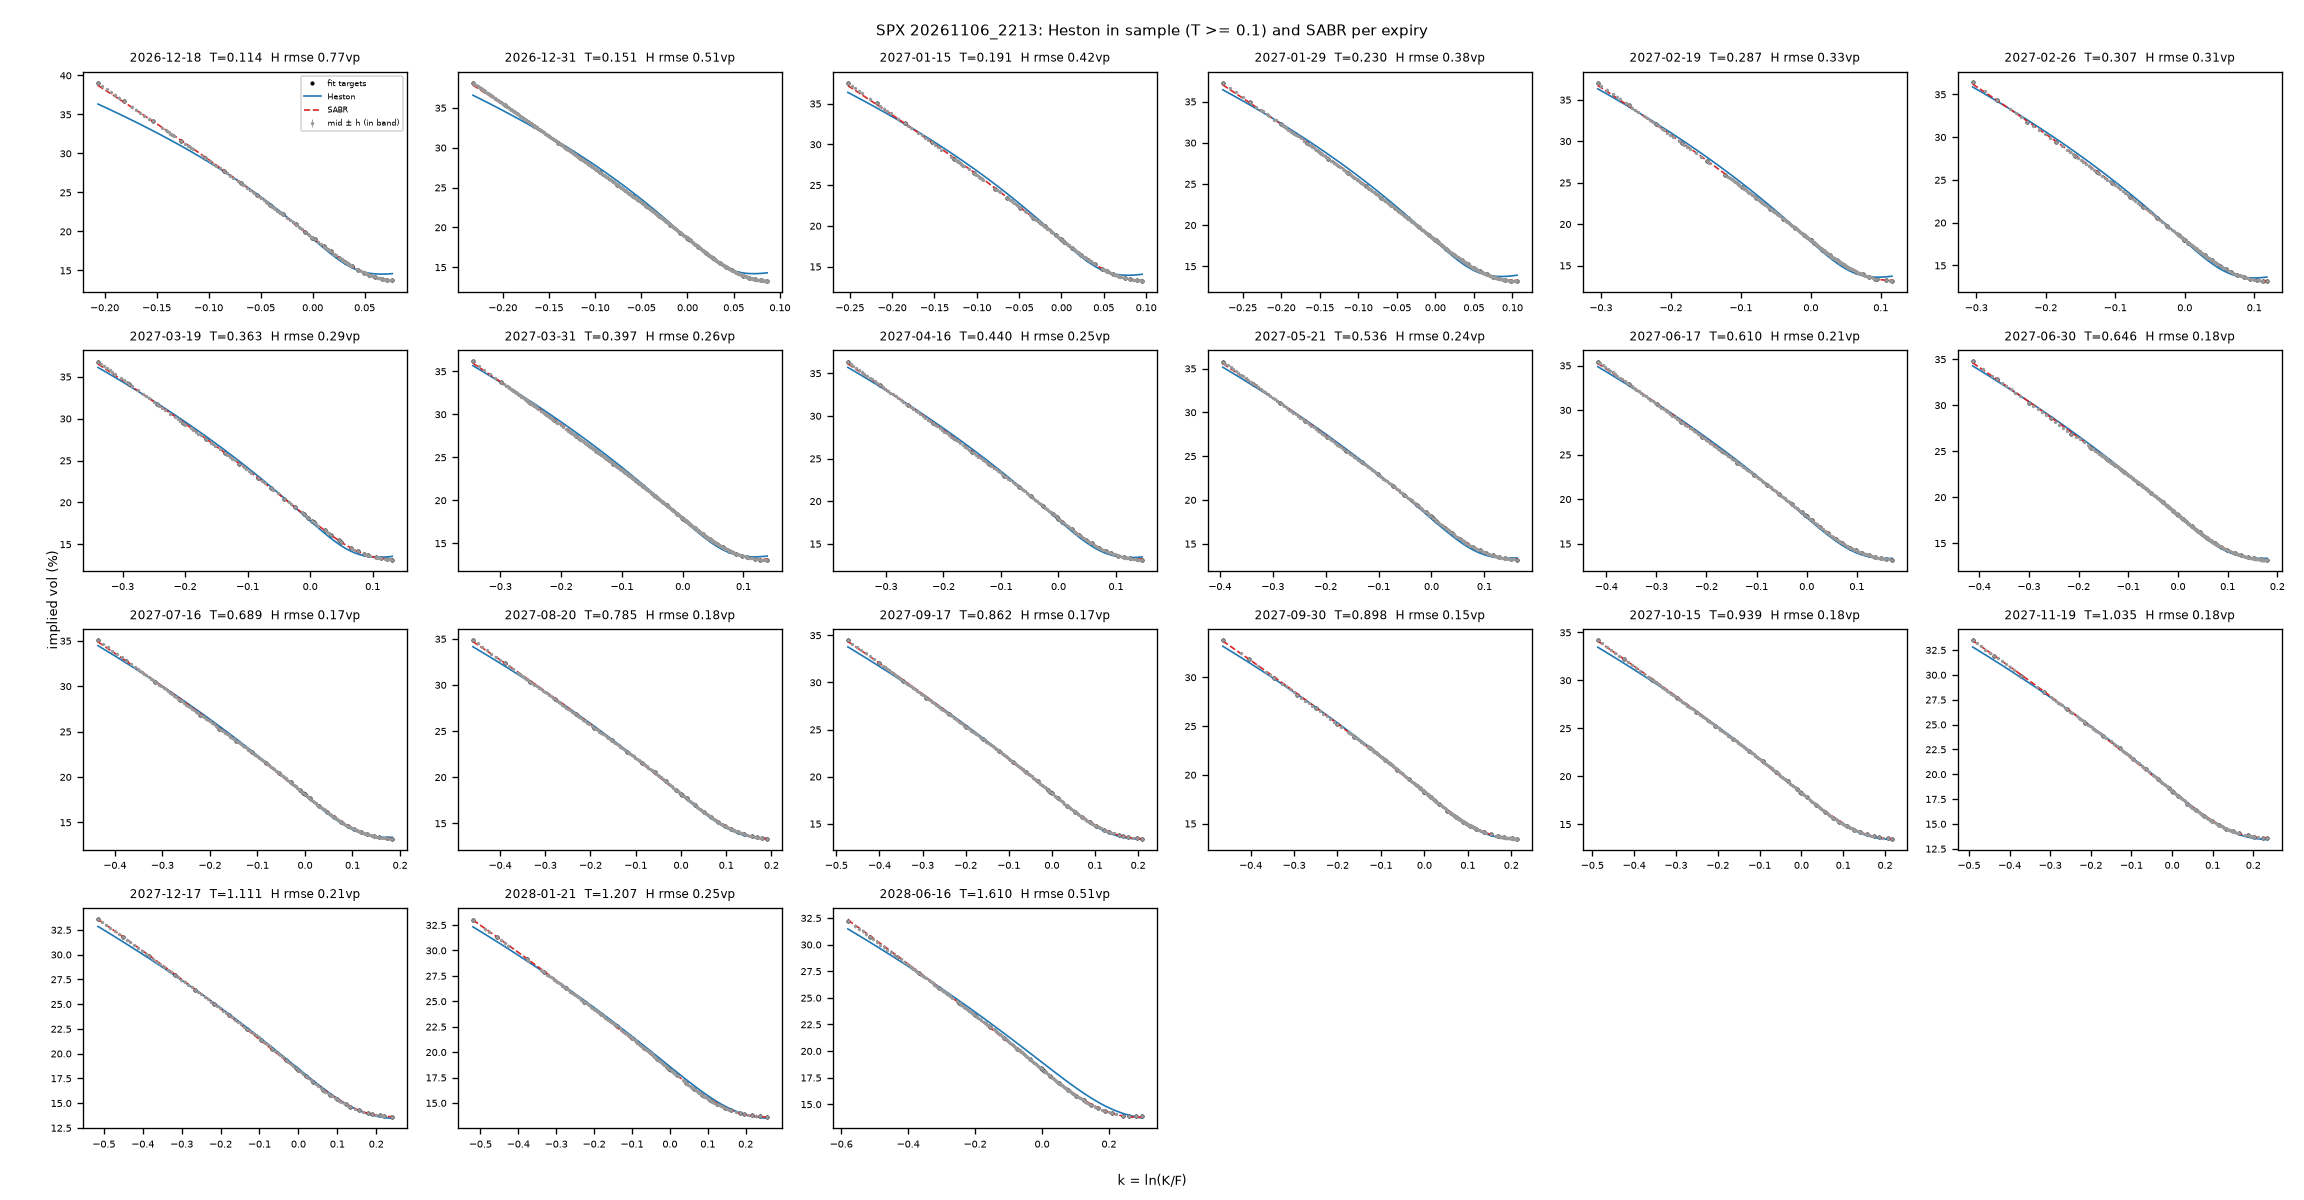
\includegraphics[width=\textwidth]{calibration_smiles_long_20261106_2213.png}
\caption{The 21 in-sample expiries. Grey dots: mids within the band with $\pm h$ bars; black dots: thinned targets;
blue line: Heston; red dashes: SABR for that expiry. The Heston RMSE is in the title.}
\label{fig:cal-long}

\bigskip
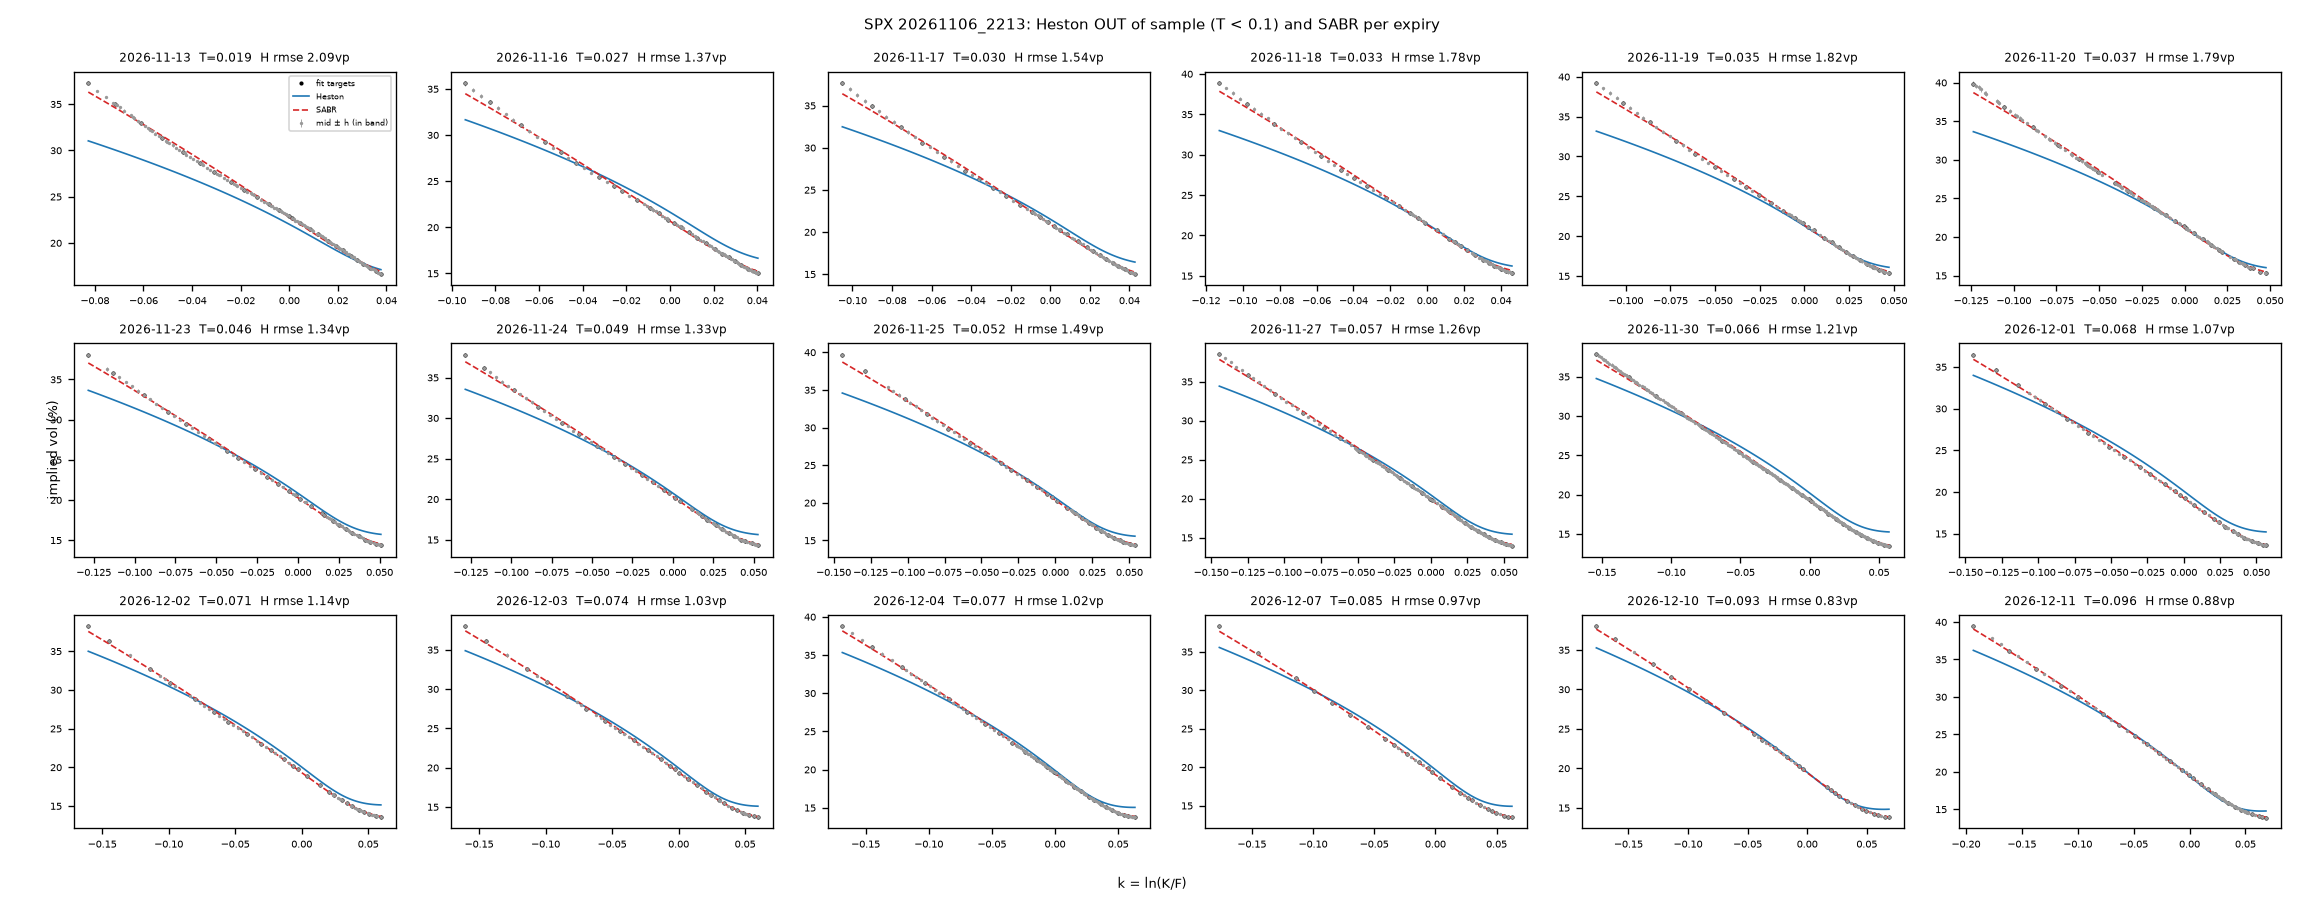
\includegraphics[width=\textwidth]{calibration_smiles_short_20261106_2213.png}
\caption{The 18 out-of-sample expiries ($T<0.1$), same legend: Heston is too flat on every weekly.}
\label{fig:cal-short}
\end{figure}

Table~\ref{tab:cal-rmse} summarizes the error. In Figure~\ref{fig:cal-long} Heston follows the central part well; the
in-sample error is U-shaped, 0.77 points on the first expiry ($T=0.114$), below 0.2 around one year, 0.51 on the last
($T=1.61$, where Heston also sits above the market at the money: 18.94\% against 18.29\%). A single $\kappa$ finds a
compromise. In Figure~\ref{fig:cal-short} the short-end failure is evident, as \eqref{eq:cal-g} predicts: Heston is too
low in the left wing and too high on the right. The worst expiry is 2026-11-13 ($T=0.019$): RMSE 2.09 and maximum
deviation 6.29 points. SABR sits on the data everywhere.

\subsection{Sensitivity: what the SEs do not say}
The last columns of Table~\ref{tab:cal-fit} redo the fit changing one choice at a time. With 50 targets per expiry
(1077 quotes) the parameters move by at most 1.06 SE; with the price objective function by at most 0.83 SE. With the
window $T\ge2$ weeks (33 expiries, 874 quotes), instead, $\kappa$ goes to 5.96 ($+12.97$ SE) and $\xi$ to 1.96
($+12.90$ SE): the short expiries ask for faster mean reversion and more vol-of-vol.

\begin{idea}[title={Key idea: estimation error versus model error}]
Curvature SEs say how narrow the minimum is \emph{if the model is right}. But $s^2=7.37$ says it is not, and the window
alone moves $\kappa$ and $\xi$ by about 13 SE: the true uncertainty is about \textbf{ten times} that of the SEs. It
should be reported as the range of the variants: $\kappa\in[4.49,5.96]$ against SE 0.107, $\xi\in[1.62,1.96]$ against
SE 0.024. ``$\kappa=4.58\pm0.11$'' would be misleading.
\end{idea}

\section{SABR expiry by expiry}
\subsection{\texorpdfstring{The fit and the cap on $\alpha$}{The fit and the cap on alpha}}
For each expiry $(\alpha,\rho,\nu)$ is calibrated with $\beta=1$, with the same residual \eqref{eq:cal-res} and the
Hagan volatility \eqref{eq:hagan} in place of the Heston one: no COS, no inversion. There are 5 starts: a seed from
the parabola \eqref{eq:sabr-taylor} fitted near the money, plus 4 Sobol points in $\rho$ and $\ln\nu$, with $\alpha$
derived from the ATM volatility.

Deriving $\alpha$ from the ATM volatility requires \eqref{eq:alpha-atm}, which for $\rho<0$ has no positive roots above
the cap \eqref{eq:tetto}. The project chooses a \emph{restriction}, not a penalty.
\begin{itemize}
\item The objective function uses $(\alpha,\rho,\nu)$ directly: \eqref{eq:alpha-atm} does not appear in it, and the cap
creates no holes in the function.
\item \eqref{eq:alpha-atm} is used only for the starts; a start without a positive root is discarded and counted.
\item Where Hagan gives \code{NaN} ($1+c_1T\le0$), TRF rejects the trial point by shrinking the trust region.
\end{itemize}

\begin{progetto}[title={In the qpricer project: SABR on the 39 expiries}]
39 fits out of 39, 0 starts discarded out of 195, no parameter at the boundary. RMSE from 0.057 to 0.307 vol points;
$\rho$ between $-0.81$ and $-0.74$. An independent check, with 9 starts of its own and without \eqref{eq:alpha-atm},
recovers the same parameters to $10^{-6}$: the restriction did not distort the fit. The SABR smiles have no calendar
or butterfly violations.
\end{progetto}

\begin{table}[htbp]
\centering
\small
\caption{SABR ($\beta=1$) on four representative expiries. RMSE in vol points.}
\label{tab:cal-sabr}
\begin{tabularx}{\textwidth}{X r r r r r r}
\toprule
expiry & $T$ & $\alpha$ & $\rho$ & $\nu$ & $\nu^2T$ & RMSE\\
\midrule
2026-11-13 & 0.019 & 0.2285 & $-0.809$ & 4.297 & 0.352 & 0.299\\
2026-12-18 & 0.114 & 0.1930 & $-0.780$ & 2.667 & 0.812 & 0.066\\
2027-05-21 & 0.536 & 0.1833 & $-0.762$ & 1.267 & 0.861 & 0.070\\
2028-06-16 & 1.610 & 0.1877 & $-0.737$ & 0.694 & 0.776 & 0.062\\
\bottomrule
\end{tabularx}
\end{table}

\subsection{\texorpdfstring{Why $\nu$ falls, and what it implies}{Why nu falls, and what it implies}}
In Table~\ref{tab:cal-sabr} $\nu$ falls from 4.30 to 0.69 while $\rho$ stays almost still. By \eqref{eq:sabr-taylor}
the SABR ATM skew is about $\tfrac12\rho\nu(1+c_1T)$ and, at fixed parameters, does not decay with $T$: SABR has no
mean reversion, and to follow the market skew the fit must lower $\nu$.

But $\nu^2T$ stays between 0.35 and 0.89 on \textbf{all} 39 expiries, above 0.16, the domain in which Chapter~\ref{cap:sabr} validated Hagan against Monte Carlo. Already at $\nu=1$ the gap was $+0.40$ vol points at $T=0.5$ and
$+0.82$ at $T=1$, at $k=-0.2$.

\begin{attenzione}[title={A parametrization, not a dynamics}]
The SABR fits are excellent \emph{interpolations} of each expiry's smile. But their parameters are not those of a SABR
dynamics that reprices those vanillas: a SABR Monte Carlo with the same $(\alpha,\rho,\nu)$ would give different
smiles. They should be read as parametrizations through the Hagan formula. And per-expiry SABR says nothing about how
the smiles connect over time: it cannot be used to price a path-dependent product.
\end{attenzione}

\paragraph{SABR on Heston smiles.} Fitting SABR to the smiles generated by Heston (set S1) on the same grid, the RMSE
grows with expiry: from 0.010 points at $T=0.019$ to 0.123 at $T=1.61$ (maximum 0.184; Spearman correlation 0.90). As
$T$ grows, Heston's mean reversion shapes the smile in a way SABR does not reproduce.

\section{No-arbitrage checks}
The filter of Chapter~\ref{cap:dati} guarantees monotonicity and vertical spreads. Here calendar and convexity are
checked as a \emph{diagnostic}.

\subsection{Calendar}
\noindent\textbf{Step 1.} With proportional dividends $X_t=S_t/F(0,t)$ is a martingale with $X_0=1$, and the
normalized undiscounted call with expiry $T$ and log-moneyness $k=\ln(K/F_T)$ is worth $\E(X_T-e^k)^+$.

\noindent\textbf{Step 2.} $x\mapsto(x-e^k)^+$ is convex; for $T_1<T_2$, conditioning on $\mathcal F_{T_1}$ and using
Jensen, $\E(X_{T_2}-e^k)^+\ge\E(X_{T_1}-e^k)^+$.

\noindent\textbf{Step 3.} The normalized call is Black as a function of $k$ and of the \textbf{total variance}
$w=\sigma^2T$, and it is increasing in $w$. Hence
\begin{equation}\label{eq:cal-calendario}
w(k,T_2)\ge w(k,T_1)\qquad\text{for } T_2>T_1,\ k\text{ fixed}.
\end{equation}
The condition is on the total variance, not on the volatility, which can fall with $T$.

For each of the 38 pairs of consecutive expiries, $w$ is interpolated linearly in $k$ between the quotes of each
expiry, only on the common interval (extrapolating would invent violations). Violation \emph{on the mid}:
$w^m_{j+1}(k)<w^m_j(k)$; \emph{strict}: $w^a_{j+1}(k)<w^b_j(k)$.

\subsection{Butterfly}
\noindent\textbf{Step 1.} For three consecutive strikes let
\[
\lambda_i=\frac{K_{i+1}-K_i}{K_{i+1}-K_{i-1}},\qquad\text{so that}\qquad K_i=\lambda_iK_{i-1}+(1-\lambda_i)K_{i+1}.
\]

\noindent\textbf{Step 2.} The ``tent'' portfolio (long $\lambda_i$ calls at $K_{i-1}$, long $1-\lambda_i$ at
$K_{i+1}$, short one at $K_i$) has payoff $\ge0$, because $K\mapsto(x-K)^+$ is convex. Hence its price is
non-negative:
\begin{equation}\label{eq:cal-butterfly}
B_i=\lambda_ic_{i-1}+(1-\lambda_i)c_{i+1}-c_i\ge0 .
\end{equation}
\noindent\textbf{Step 3.} In the limit of dense strikes this is $\partial^2C/\partial K^2\ge0$: by
Breeden--Litzenberger \eqref{eq:breeden}, a non-negative density.

The undiscounted calls are built by parity, $c_i=V_i/\DF+(F-K_i)^+$; parity adds a function linear in $K$ that
vanishes from $B_i$, except in the triples straddling $F$. Violation \emph{on the mid}: $B^m_i<0$; \emph{strict}:
\[
\lambda_ic^a_{i-1}+(1-\lambda_i)c^a_{i+1}-c^b_i<0,
\]
that is, buying the wings at the ask and selling the body at the bid would give a credit. Size: $z_i=-B^m_i/h^B_i$,
with $h^B_i$ the half-spread of the butterfly.

\begin{progetto}[title={In the qpricer project: the SPX surface}]
\begin{itemize}
\item \textbf{Calendar}: 11{,}054 points, 0 violations on the mid, 0 strict.
\item \textbf{Butterfly}: 7547 triples, \textbf{2126 violations on the mid}, \textbf{0 strict}, maximum $z$ 0.43:
every shortfall on the mid is less than half the butterfly half-spread, hence inside the spreads.
\end{itemize}
The checks have power: a flat surface gives 0 violations, a mid raised by 3 half-spreads and two swapped smiles are
flagged, the Heston S1 surface has no strict violations.
\end{progetto}

\begin{attenzione}
With strikes 5 points apart the butterfly is tiny and its mid is quoting noise. The correct statement is: ``no
calendar or convexity arbitrage is tradable at bid/ask prices''.
\end{attenzione}

\section{The link with the autocallable}
The file \code{data/processed/heston\_fit\_20261106\_2213.json} contains $\hat p$ with SEs and provenance, and Chapter~\ref{cap:autocallable} uses it to price the autocallables. The window $T\ge0.1$ covers the dates of \mbox{AC-Q} (up to
1.5 years), while \mbox{AC-A} (3 years) is an extrapolation beyond the last quoted expiry. On \mbox{AC-Q} Heston is
worth 1.87\% of notional less than Black ($-0.018688$, CRN SE 0.000217) and the par coupon rises from 5.60\% to
8.93\%; the dominant term is the skew at the 60--70\% barriers, the part of the smile that the calibration fits. Two
caveats: Black is evaluated at the ATM volatility of calibrated Heston (18.85\%), not at the market one (18.29\%); and
the window uncertainty ($\kappa$ and $\xi$ moved by about 13 SE) has not been propagated to the autocallable price.

\needspace{6\baselineskip}
\begin{riassunto}
\begin{itemize}
\item Targets: OTM volatilities in the 5$\Delta$ band, thinned to 25--27 per expiry; volatility residuals weighted by
$1/\max(h,0.001)$, equivalent at first order to prices weighted by $1/\vega^2$.
\item Heston on $T\ge0.1$, the rest out of sample: Heston has a single clock, $1/\kappa$.
\item COS frozen at $(16384,64)$ with an a-priori budget of $10^{-5}$ in market vega (measured $9.21\times10^{-6}$),
which is not a volatility accuracy. Narrowed box; on the original box 20 starts out of 20 find the same optimum.
\item Synthetic test S1, S2: tolerances from the sandwich before the fit, G1--G4 passed; expected false alarms about 8\%.
\item SPX: $\hat p=(0.052372,\,4.5751,\,0.052925,\,1.6477,\,-0.75180)$, $\nu_F=0.178$. RMSE 0.328 vol points in sample,
1.379 out of sample. The SEs underestimate the uncertainty by a factor of about ten.
\item SABR: RMSE 0.057--0.307, but $\nu^2T$ between 0.35 and 0.89: parametrizations, not dynamics.
\item No tradable arbitrage; 2126 negative butterflies on the mid, all inside the spreads.
\end{itemize}
\end{riassunto}

\needspace{6\baselineskip}
\begin{domande}
\begin{enumerate}
\item In what sense do volatility residuals and prices divided by vega coincide at first order? Why are volatilities
preferred?
\item Why does a COS that chooses $(N,L)$ by itself ruin a finite-difference Jacobian?
\item How do you show that narrowing the constraints did not change the result?
\item What is the $\kappa$--$\theta$ ridge, and why does it not show up on this window?
\item Why can Heston not fit weeklies and long expiries together? \emph{Hint:} \eqref{eq:cal-g}.
\item The SEs say $\kappa=4.58\pm0.11$: what do you report instead?
\item Why does the SABR $\nu$ fall with $T$, and what does $\nu^2T>0.16$ imply?
\item Derive the calendar and butterfly conditions. What is the difference between a violation on the mid and a strict
one?
\end{enumerate}
\end{domande}
